\documentclass[12pt]{article}
\usepackage[left=1cm, right=1cm, top=2cm,bottom=1.5cm]{geometry} 

\usepackage[parfill]{parskip}
\usepackage[utf8]{inputenc}
\usepackage[T2A]{fontenc}
\usepackage[russian]{babel}
\usepackage{enumitem}
\usepackage[normalem]{ulem}
\usepackage{amsfonts, amsmath, amsthm, amssymb, mathtools}
\usepackage{tabularx}
\usepackage{hhline}

\usepackage{accents}
\usepackage{fancyhdr}
\pagestyle{fancy}
\renewcommand{\headrulewidth}{1.5pt}
\renewcommand{\footrulewidth}{1pt}

\usepackage{graphicx}
\usepackage[figurename=Рис.]{caption}
\usepackage{subcaption}
\usepackage{float}

%%Наименование папки откуда забирать изображения
\graphicspath{ {./images/} }

%%Изменение формата для ввода доказательства
\renewcommand{\proofname}{$\square$  \nopunct}
\renewcommand\qedsymbol{$\blacksquare$}

%%Изменение отступа на таблицах
\addto\captionsrussian{%
	\renewcommand{\proofname}{$\square$ \nopunct}%
}
%% Римские цифры
\newcommand{\RN}[1]{%
	\textup{\uppercase\expandafter{\romannumeral#1}}%
}

%% Для удобства записи
\newcommand{\MR}{\mathbb{R}}
\newcommand{\MQ}{\mathbb{Q}}
\newcommand{\MN}{\mathbb{N}}
\newcommand{\MTB}{\mathbb{T}}
\newcommand{\MI}{\mathrm{I}}
\newcommand{\MJ}{\mathrm{J}}
\newcommand{\MH}{\mathrm{H}}
\newcommand{\MT}{\mathrm{T}}
\newcommand{\MU}{\mathcal{U}}
\newcommand{\MV}{\mathcal{V}}
\newcommand{\MW}{\mathcal{W}}
\newcommand{\VN}{\varnothing}
\newcommand{\VE}{\varepsilon}

\theoremstyle{definition}
\newtheorem{defn}{Опр:}
\newtheorem{rem}{Rm:}
\newtheorem{prop}{Утв.}
\newtheorem{exrc}{Упр.}
\newtheorem{lemma}{Лемма}
\newtheorem{theorem}{Теорема}
\newtheorem{corollary}{Следствие}

\newenvironment{cusdefn}[1]
{\renewcommand\thedefn{#1}\defn}
{\enddefn}

\DeclareRobustCommand{\divby}{%
	\mathrel{\text{\vbox{\baselineskip.65ex\lineskiplimit0pt\hbox{.}\hbox{.}\hbox{.}}}}%
}
%Короткий минус
\DeclareMathSymbol{\SMN}{\mathbin}{AMSa}{"39}
%Длинная шапка
\newcommand{\overbar}[1]{\mkern 1.5mu\overline{\mkern-1.5mu#1\mkern-1.5mu}\mkern 1.5mu}
%Функция знака
\DeclareMathOperator{\sgn}{sgn}

%Функция ранга
\DeclareMathOperator{\rk}{\text{rk}}

%Обозначение константы
\DeclareMathOperator{\const}{\text{const}}

%Интеграл в большом формате
\DeclareMathOperator{\dint}{\displaystyle\int}
\newcommand{\ddint}[2]{\displaystyle\int\limits_{#1}^{#2}}

\newcommand{\smallerrel}[1]{\mathrel{\mathpalette\smallerrelaux{#1}}}
\newcommand{\smallerrelaux}[2]{\raisebox{.1ex}{\scalebox{.75}{$#1#2$}}}

\newcommand{\smallin}{\smallerrel{\in}}
\newcommand{\smallnotin}{\smallerrel{\notin}}

\newcommand*{\medcap}{\mathbin{\scalebox{1.25}{\ensuremath{\cap}}}}%
\newcommand*{\medcup}{\mathbin{\scalebox{1.25}{\ensuremath{\cup}}}}%

\makeatletter
\newcommand{\vast}{\bBigg@{3.5}}
\newcommand{\Vast}{\bBigg@{5}}
\makeatother

%Промежуточное значение для sup\inf, поскольку они имеют разную высоту
\newcommand{\newsup}{\mathop{\smash{\mathrm{sup}}}}
\newcommand{\newinf}{\mathop{\mathrm{inf}\vphantom{\mathrm{sup}}}}

%Скалярное произведение
\DeclarePairedDelimiterX{\inner}[2]{\langle}{\rangle}{#1, #2}

%Подпись символов снизу
\newcommand{\ubar}[1]{\underaccent{\bar}{#1}}

%% Шапка для букв сверху
\newcommand{\wte}[1]{\widetilde{#1}}

\begin{document}
\lhead{Математический анализ - \RN{2}}
\chead{Шапошников С.В.}
\rhead{Лекция - 25}

\section*{Критерий Лебега}
\begin{defn}
	Множество $E \subset \MR$ называется \uwave{множеством меры ноль по Лебегу}, если: $\forall \VE > 0, \, \exists$ не более чем счетный набор интервалов (или отрезков) $\{\MI_n\}$ таких, что:
	\begin{enumerate}[label={(\arabic*)}]
		\item Множество $E$ покрыто этими интервалами: $E \subset \displaystyle \bigcup\limits_n \MI_n$;
		\item Сумма длин этих интервалов меньше $\VE$: $\displaystyle \sum\limits_{n} |\MI_n| < \VE$;
	\end{enumerate}
\end{defn}
\begin{defn}
	Если некоторое свойство имеет место для всех точек, кроме множества меры ноль, то говорят, что это \uwave{свойство выполняется почти всюду}.
\end{defn}
\begin{theorem}(\textbf{Критерий Лебега})
	$f$ - интегрируема по Риману на отрезке $[a,b] \Leftrightarrow f$ - ограничена на отрезке $[a,b]$ и $f$ почти всюду непрерывна на отрезке $[a,b]$.
\end{theorem}
\begin{rem}
	Проще говоря, функция интегрируема тогда и только тогда, когда функция ограничена, а множество точек разрыва является множеством меры ноль по Лебегу.
\end{rem}
\begin{proof}
	Рассматриваем только ограниченную функцию $f$.
	
	$(\Rightarrow)$ Пусть $f$ - интегрируема на $[a,b]$, тогда выполняется критерий Дарбу:
	$$
		\forall \VE > 0, \, \exists \, \MTB \colon \sum\limits_{k}\omega(f,\Delta_k){\cdot}|\Delta_k| < \VE
	$$
	\uline{Напоминание про непрерывность}: $\omega(f,a) = \lim\limits_{\delta \to 0+} \omega\left(f, \MU_\delta(a)\right)$ - это колебание функции $f$ в точке $a$. Мы знаем, что $f$ - непрерывна в точке $a \Leftrightarrow \omega(f,a) = 0$. Множество точек разрыва замкнуто и равно:
	$$
		\bigcup\limits_{n} \left\{x \colon \omega(f,x) \geq \dfrac{1}{n}\right\}
	$$
	Таким образом, достаточно показать, что $\forall n \in \MN$ множество 
	$$
		E_n = \left\{x \colon \omega(f,x) \geq \dfrac{1}{n}\right\}
	$$
	является множеством меры ноль по Лебегу, поскольку счетное объединение множества меры ноль будет также множеством меры ноль (см. свойство $3$ на прошлой лекции). Фиксируем $n$ и рассмотрим множество $E_n$. Пусть $\VE > 0$, тогда $\exists \, \MTB$ - разбиение отрезка $[a,b]$ на отрезки $\Delta_k$:
	$$
		\sum\limits_k \omega(f,\Delta_k){\cdot}|\Delta_k| < \VE
	$$
	Пусть $\Delta_k \cap E_n \neq \VN$, то есть $\exists \, a \in E_n \colon a \in \Delta_k$, тогда возможно несколько исходов:
	\begin{enumerate}[label={(\arabic*)}]
		\item $a$ лежит внутри $\Delta_k$, тогда по определению колебания в точке верно: 
		$$
			\omega(f,\Delta_k) = \sup\limits_{x,y\smallin \Delta_k}|f(x) - f(y)| \geq \omega\left(f, \MU_\delta(a)\right) = \sup\limits_{x,y\smallin \MU_\delta(a)}|f(x) - f(y)| \Rightarrow \omega(f,\Delta_k) \geq \omega(f,a) \geq \dfrac{1}{n}
		$$
		\item $a \in \Delta_k \cap \Delta_{k+1}$ или $a \in \Delta_k \cap \Delta_{k-1}$. Рассмотрим случай $a \in \Delta_k \cap \Delta_{k+1}$. Хотя бы для одного из отрезков $\Delta_k, \, \Delta_{k+1}$ колебание не будет маленьким: 
		$$
			\omega(f,\Delta_k) \geq \dfrac{1}{3n} \vee \omega(f,\Delta_{k+1}) \geq \dfrac{1}{3n}
		$$ 
		На обоих отрезках колебание не может оказаться маленьким, иначе получим противоречие: 
		$$
			\omega(f,\Delta_k) < \dfrac{1}{3n} \wedge \omega(f,\Delta_{k+1}) < \dfrac{1}{3n} \Rightarrow \omega(f,a) \leq \dfrac{2}{3n}
		$$
		Почему это так? Пусть $x,y \in \MU_\delta(a)$, тогда рассмотрим разность функции $f$ в этих точках:
		$$
			|f(x) - f(y)| \leq |f(x) - f(a)| + |f(y) - f(a)| \leq \omega(f,\Delta_k) + \omega(f,\Delta_{k+1}), \, x \in \Delta_k, \, y \in \Delta_{k+1}
		$$
		$$
			|f(x) - f(y)| \leq \omega(f,\Delta_k), \, x,y \in \Delta_k
		$$
		$$
			|f(x) - f(y)| \leq \omega(f,\Delta_{k+1}), \, x,y \in \Delta_{k+1}
		$$
	\end{enumerate}
	Таким образом, если каждое колебание маленькое, то верно следующее:
	$$
		|f(x) - f(y)| \leq \dfrac{2}{3n} \Rightarrow \omega(f,a) \leq \dfrac{2}{3n} < \dfrac{1}{n}
	$$
	Получили противоречие с тем, что $a \in E_n$. Значит, хотя бы на одном из отрезков колебание не меньше, чем $\tfrac{1}{3n}$. 
	
	Итог: если возьмем объединение отрезков на которых колебание больше, чем $\tfrac{1}{3n}$, то оно заведомо будет содержать $E_n$:
	$$
		\MI = \left\{k\colon \omega(f,\Delta_k) \geq \dfrac{1}{3n}\right\}, \, E_n \subset \bigcup\limits_{k\smallin \MI}\Delta_k
	$$
	Рассмотрим следующую сумму:
	$$
		\sum\limits_{k \smallin \MI}|\Delta_k| = 3n \sum\limits_{k \smallin \MI}\dfrac{1}{3n}|\Delta_k| \leq 3n \sum\limits_{k \smallin \MI}\omega(f,\Delta_k){\cdot}|\Delta_k| \leq 3n \sum\limits_{k }\omega(f,\Delta_k){\cdot}|\Delta_k| < 3n\VE
	$$
	Поскольку $\VE > 0$ - произвольное, то мы накрыли множество $E_n$ конечным набором отрезков, сумму длин которых можно сделать сколь угодно маленькой. Следовательно, $E_n$ - множество меры ноль.
	
	$(\Leftarrow)$ Пусть $f$ - ограничена на $[a,b]$ и почти всюду непрерывна на $[a,b]$. Будем проверять критерий Дарбу:
	$$
		\forall \VE > 0, \, \exists \, \MTB \colon \sum\limits_{k}\omega(f,\Delta_k){\cdot}|\Delta_k| < \VE
	$$
	Но перед этим, вспомним лемму из прошлой лекции:
	\begin{lemma}
		Если $[a,b] \subset \displaystyle \bigcup\limits_n \MI_n$, где $\MI_n$ - интервалы, то верно следующее: 
		$$
			b - a \leq \displaystyle \sum\limits_n |\MI_n \cap [a,b]| \leq \displaystyle \sum\limits_n |\MI_n|
		$$	
	\end{lemma}
	и докажем новую лемму:
	\begin{lemma}
		Пусть $\MI$ - ограниченный промежуток (интервал, отрезок, полуинтервал) и $\MJ_1, \dotsc \MJ_M$ - промежутки, причем $\forall k,m, \, \MJ_k$ и $\MJ_m$ либо не пересекаются, либо пересекаются по концам ($\forall k,m , \, \mathring{\MJ}_k \cap \mathring{\MJ}_m = \VN$). Тогда верно следующее: 
		$$
			\displaystyle \bigcup\limits_{k = 1}^M \MJ_k \subset \MI \Rightarrow \sum\limits_{k = 1}^M|\MJ_k| \leq |\MI|
		$$
	\end{lemma}
	\begin{figure}[H]
		\centering
		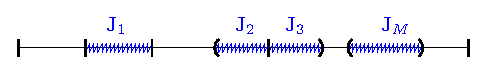
\includegraphics[width=0.55\textwidth]{25_1.eps}
		\label{25_1}
		\caption{Набор промежутков внутри ограниченного промежутка.}
		\label{fig:Ограниченный промежуток}
	\end{figure}
	\begin{proof}
		Докажем по индукции:
		
		\textbf{\uline{База}}: $M = 1 \Rightarrow \MJ_1 \subset \MI \Rightarrow |\MJ_1| \leq |\MI|$, поскольку $\MJ_1 = ]\gamma,\delta[ \subset \MI = ]\alpha,\beta[ \Rightarrow \alpha \leq \gamma \leq \delta \leq \beta \Rightarrow \delta - \gamma \leq \beta - \alpha$.
		
		\textbf{\uline{Шаг}}: Пусть доказано для $M$, докажем для $M+1$. Будем считать, что $\MJ_k = ]\alpha_k, \beta_k[, \, \MI = ]\alpha,\beta[$. Перенумеровывая, если нужно, $\MJ_k$ будем считать, что $\alpha_{M+1} = \max\limits_{k}\alpha_k$ и автоматически получим $\beta_{M+1} = \max\limits_{k}\beta_k$. Таким образом, берем самый правый промежуток. По построению: 
		$$
			\displaystyle \bigcup\limits_{k = 1}^M \MJ_k \subset ]\alpha, \alpha_{M+1}[ \Rightarrow\sum\limits_{k = 1}^M |\MJ_k| \leq \alpha_{M+1} - \alpha
		$$
		где последнее неравенство выполненно по предположению индукции. Добавим к нему длину последнего промежутка $\MJ_{M+1}$:
		$$
			\sum\limits_{k = 1}^M |\MJ_k| + (\beta_{M+1} - \alpha_{M+1}) = \sum\limits_{k = 1}^{M+1} |\MJ_k| \leq \alpha_{M+1} - \alpha + (\beta_{M+1} - \alpha_{M+1}) = \beta_{M+1} - \alpha \leq \beta - \alpha = |\MI|
		$$
		Таким образом, получили требуемое по индукции.
	\end{proof}
	Пусть $E$ - множество точек разрыва. Так как по условию $E$ это множество меры ноль, то верно:
	$$
		\forall \VE > 0, \, \exists \, \{\MI_j \}\colon \sum\limits_{j}|\MI_j| < \VE, \, E \subset \bigcup\limits_j \MI_j
	$$
	Если точка $x \notin E$, то $f$ непрерывна в ней $\Rightarrow \exists \, \MU_{\delta_x}(x) \colon \omega\left(f,\MU_{3\delta_x}(x)\right) < \VE$, то есть $\delta_x$ выбрано так, чтобы в утроенной окрестности колебание было меньше, чем $\VE$ (это можно сделать из-за непрерывности). Тогда будет верно:
	$$
		[a,b] \subset \bigcup\limits_j \MI_j \bigcup\limits_{x \smallnotin E} \MU_{\delta_x}
	$$
	Но это всё - открытые множества $\Rightarrow$ мы можем выбрать конечное подпокрытие, поскольку отрезок $[a,b]$ это компакт:
	$$
		\MU_{\delta_1}, \dotsc, \MU_{\delta_M}, \MI_1, \dotsc , \MI_N \Rightarrow [a,b] \subset \bigcup\limits_{j = 1}^{N} \MI_j \bigcup\limits_{i = 1}^M \MU_{\delta_i}
	$$
	Выберем $\delta = \min\{\delta_1, \dotsc, \delta_M\}$ и разбиение $\MTB$ с масштабом $\lambda(\MTB) < \delta$. Будем рассматривать следующую сумму:
	$$
		\sum\limits_{k}\omega\left(f, \Delta_k\right){\cdot}|\Delta_k|
	$$
	\newpage
	Понятно, что есть два типа точек в этой сумме: 
	\begin{enumerate}[label={\arabic*)}]
		\item точки, которые попадают в окрестности $\MU_{\delta_i}$ (тут маленькие колебания);
		\item точки, которые закрыты интервалами $\MI_j$ (тут маленькая длина интервалов);
	\end{enumerate}
	Рассмотрим множество отрезков $\Delta_k$, которые пересекаются с множествами $\MU_{\delta_i}$ и которые не имеют с ними общих точек. Обозначим их как $\mathrm{K}$ и $\mathrm{R}$ соответственно:
	$$
		\mathrm{K} = \left\{k \colon \Delta_k \cap \bigcup\limits_{i=1}^{M} \MU_{\delta_i} \neq \VN \right\}, \, \mathrm{R} = \left\{k \colon \Delta_k \cap \bigcup\limits_{i=1}^{M} \MU_{\delta_i} = \VN \right\}
	$$
	Разделим рассматриваемую сумму на две соответствующие части:
	$$
		\sum\limits_{k}\omega\left(f, \Delta_k\right){\cdot}|\Delta_k| = \sum\limits_{k \smallin \mathrm{K}}\omega\left(f, \Delta_k\right){\cdot}|\Delta_k| + \sum\limits_{k \smallin \mathrm{R}}\omega\left(f, \Delta_k\right){\cdot}|\Delta_k|
	$$
	Рассмотрим случай, когда $\Delta_k \cap \MU_{\delta_i} \neq \VN$. Пусть $\MU_{\delta_i} = (a_i - \delta_i, a_i + \delta_i)$, где $a_i$ - середина окрестности $\MU_{\delta_i}$.
	\begin{figure}[H]
		\centering
		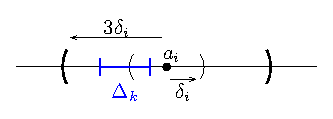
\includegraphics[width=0.35\textwidth]{25_2.eps}
		\label{25_2}
		\caption{Пересечение $\Delta_k$ с $\MU_{\delta_i}$ не пусто.}
		\label{fig:Случай пересечения точек 1}
	\end{figure}
	Тогда $\Delta_k \subset \MU_{3\delta_i}$, поскольку от любой точки отрезка $\Delta_k$ до $a_i$ расстояние не больше, чем $\delta_i$ и длина отрезка $\Delta_k$ не больше, чем $\delta < \delta_i$. Таким образом, получим:
	$$
		\Delta_k \subset \MU_{3\delta_i} \Rightarrow \omega(f,\Delta_k) < \VE \Rightarrow \sum\limits_{k \smallin \mathrm{K}}\omega\left(f, \Delta_k\right){\cdot}|\Delta_k| < \VE{\cdot}\!\sum\limits_{k \smallin \mathrm{K}}|\Delta_k|\leq \VE(b-a)
	$$
	Рассмотрим случай, когда $\Delta_k \cap \MU_{\delta_i} = \VN$. Поскольку весь отрезок $[a,b]$ покрыт конечным набором окрестностей $\MU_{\delta_i}$ и интервалов $\MI_j$, то такие $\Delta_k$ содержатся в объединении интервалов $\MI_j$:
	$$
		\Delta_k \subset \bigcup\limits_{j = 1}^N \MI_j 
	$$
	В противном случае, была бы точка отрезка, которая ничем не закрыта $\Rightarrow$ противоречие с построением конечного покрытия. Пусть $\overline{M} = \sup\limits_{[a,b]}|f|$, распишем вторую сумму:
	$$
		\sum\limits_{k \smallin \mathrm{R}}\omega\left(f, \Delta_k\right){\cdot}|\Delta_k| \leq 2\overline{M} {\cdot}\! \sum\limits_{k \in \mathrm{R}}|\Delta_k| \leq 2\overline{M} {\cdot}\! \sum\limits_{k \smallin \mathrm{P}}|\Delta_k|, \, \mathrm{P} = \left\{k \colon \Delta_k \subset\bigcup\limits_{j = 1}^N \MI_j  \right\}
	$$
	Поскольку отрезок $\Delta_k$ закрыт интервалами, то можем применить первую лемму:
	$$
		2\overline{M} {\cdot}\! \sum\limits_{k \smallin \mathrm{P}}|\Delta_k| \leq 2\overline{M} {\cdot}\! \sum\limits_{k \smallin \mathrm{P}} \sum\limits_{j = 1}^N|\Delta_k \cap \MI_j| \leq 2 \overline{M} \sum\limits_{k}\sum\limits_{j = 1}^N |\Delta_k \cap \MI_j| = 2 \overline{M} \sum\limits_{j = 1}^N\left(\sum\limits_{k} |\Delta_k \cap \MI_j|\right)
	$$
	Заметим, что $\forall k, \, \Delta_k \cap \MI_j$ - это промежутки в интервале $\MI_j$ и они могут пересекаться только концами. Тогда применяя вторую лемму к суммам внутри скобок и вспоминая, что $\MI_j$ накрывают множество меры ноль, получим:
	$$
		2 \overline{M} \sum\limits_{j = 1}^N\left(\sum\limits_{k} |\Delta_k \cap \MI_j|\right) \leq 2 \overline{M} \sum\limits_{j = 1}^N |\MI_j| < 2\overline{M} \VE
	$$
	Итог: 
	$$
		\sum\limits_{k}\omega\left(f, \Delta_k\right){\cdot}|\Delta_k| = \sum\limits_{k \smallin \mathrm{K}}\omega\left(f, \Delta_k\right){\cdot}|\Delta_k| + \sum\limits_{k \smallin \mathrm{R}}\omega\left(f, \Delta_k\right){\cdot}|\Delta_k| \leq \VE(b-a) + 2\overline{M}\VE = \VE(b-a + 2\overline{M})
	$$	
	где $(b-a + 2\overline{M})$ - это константа, а $\VE > 0$ могли взять сколь угодно маленьким $\Rightarrow$ критерий Дарбу выполнен $\Rightarrow$ функция $f$ интегрируема на $[a,b]$.
\end{proof}

\section*{Следствия критерия Лебега}
\begin{corollary}
	Пусть $f$ интегрируема по Риману на отрезке $[a,b]$ и функция $\varphi$ - непрерывна на $[m,M]$, где $m = \newinf\limits_{[a,b]}f$, $M = \sup\limits_{[a,b]}f$. Тогда $\varphi\left(f(x)\right)$ интегрируема по Риману на отрезке $[a,b]$.
\end{corollary}
\begin{proof}
	Функция $\varphi$ - непрерывна на отрезке $[m,M] \Rightarrow$ ограничена $\Rightarrow \varphi(f)$ - ограничена. Если $f$ - непрерывна в точке $x \in [a,b]$, то $\varphi\left(f\right)$ - непрерывна в точке $x \in [a,b]$, как композиция непрерывных функций. Подмножества точек разрыва больше не станет $\Rightarrow \varphi(f)$ почти всюду непрерывна.
\end{proof}
\textbf{Пример}: Если $f$ - интегрируема, то $|f|$ - интегрируема и верно следующее:
$$
	\left| \ddint{a}{b}f(x)dx \right| \leq \ddint{a}{b}|f(x)|dx
$$
Содержательно, $|f| = \varphi(f)$ - непрерывная функция, где $\varphi(t) = |t|$. Оценка интеграла справделива из монотонности: $-|f| \leq f \leq |f| \Rightarrow$ интегрируем и получаем оценку, написанную выше.

\begin{corollary}
	Если $f$ и $g$ интегрируемы по Риману на $[a,b]$, то $f{\cdot}g$ - интегрируема по Риману на $[a,b]$.
\end{corollary}
\begin{proof}
	Произведение ограниченных фукнций - ограниченная функция. Множество точек разрыва функции $f$ и $g$ - это множество меры ноль, их объединение будет также множеством меры ноль. В точках непрерывности $f$ и $g$ произведение $f{\cdot}g$ будет также непрерывным $\Rightarrow f{\cdot}g$ непрерывно почти всюду $\Rightarrow$ интегрируемо по критерию Лебега.
\end{proof}

\begin{theorem}(\textbf{Теорема о среднем})
	Пусть $f$ и $g$ - интегрируемы на $[a,b]$, $g \geq 0$, точная верхняя и нижняя грани функции $f$ равны: $m = \newinf\limits_{[a,b]}f$, $M = \sup\limits_{[a,b]}f$. Тогда: 
	$$
		\exists \, \mu \in [m,M] \colon \ddint{a}{b}f(x){\cdot}g(x)dx = \mu\ddint{a}{b}g(x)dx
	$$
	Более того, если $f$ - непрерывная, то $\mu = f(c)$, где $c \in [a,b]$.
\end{theorem}
\begin{proof}
	Из интегрируемости $f$ и $g$ получаем интегрируемость $f{\cdot}g$ и применяем первую теорему о среднем для интегралов (см. лекцию $23$).
\end{proof}

\begin{corollary}\hfill
	\begin{enumerate}[label={\arabic*)}]
		\item Если $f$ интегрируема на $[a,b]$ и отрезок $[c,d] \subset [a,b]$, то $f$ интегрируема на $[c,d]$;
		\item Если $f$ интегрируема на $[a,c]$ и $[c,b]$, то $f$ интегрируема на $[a,b]$;
	\end{enumerate}
\end{corollary}
\begin{proof}\hfill
	\begin{enumerate}[label={\arabic*)}]
		\item Функция ограниченная на $[a,b]$ будет ограниченной на любом подотрезке. 
		
		Множество точек разрыва $f$ на $[a,b]$ - это множество меры ноль, а множество точек разрыва на $[c,d]$ будет подмножеством этого множества меры ноль $\Rightarrow f$ непрерывна на $[c,d]$ почти всюду.
		
		Применяем критерий Лебега и получаем требуемое;
		\item Если $f$ интегрируема на $[a,c]$ и $[c,b] \Rightarrow$ ограничена на обоих отрезках, тогда возьмем самое большое ограничение и получим ограниченность на $[a,b]$. 
		
		На обоих отрезках функция $f$ почти всюду непрерывна, объединение множеств меры ноль этих отрезков будет множеством меры ноль. Если $f$ была непрерывной в точке $c$ на одном отрезке, то и на другом она будет непрерывной в точке $c$, поскольку функция одна и та же.
		
		Применяем критерий Лебега и получаем требуемое;
	\end{enumerate}
\end{proof}

\begin{corollary}
	Пусть $f$ интегрируема по Риману на $[a,b]$ и $f \geq 0$. Если $\ddint{a}{b}f(x)dx = 0$, то $f =0$ п.в.
\end{corollary}
\begin{proof}
	Докажем, что $f = 0$ во всех точках непрерывности (т.е. $f \neq 0$ только на множестве меры ноль). Пусть $f(c) > 0$ и $c$ - точка непрерывности функции $f$ (не равная $a$ или $b$, на множество меры ноль это не скажется), тогда по теореме об отделимости:
	$$
		\exists \, \Delta \subset [a,b] \colon c \in \Delta,\, c \neq a \wedge c \neq b, \, f(x) \geq \dfrac{f(c)}{2}, \, \forall x \in \Delta
	$$
	Заметим, что $|\Delta| > 0$, поскольку длина отрезка - положительная величина и выполняется следующее:
	$$
		f(x) \geq \dfrac{f(c)}{2}{\cdot}\mathbb{I}_\Delta(x), \, \forall x \in [a,b]
	$$ 
	Следовательно, интегрируя неравенство, по свойству монотонности мы получим:
	$$
		\ddint{a}{b}f(x)dx \geq \dfrac{f(c)}{2}{\cdot}|\Delta| > 0
	$$
	Получили противоречие с тем, что интеграл на всем отрезке равен $0 \Rightarrow f$ принимает значение $0$ во всех точках непрерывности, то есть $f = 0$ почти всюду.
\end{proof}
\newpage
\begin{corollary}\hfill
	\begin{enumerate}[label={\arabic*)}]
		\item Пусть функции $f$ и $g$ интегрируемы по Риману на $[a,b]$ и $f = g$ почти всюду. Тогда:
		$$
			\ddint{a}{b}f(x)dx = \ddint{a}{b}g(x)dx
		$$
		\item Если функция $f$ интегрируема по Риману на $[a,b]$ и $g = f$ всюду, кроме конечного числа точек, то функция $g$ - интегрируема на $[a,b]$ и справедливо следующее:
		$$
			\ddint{a}{b}f(x)dx = \ddint{a}{b}g(x)dx
		$$
	\end{enumerate}
\end{corollary}
\begin{rem}
	Стоит обратить внимание, что если не требовать, чтобы функция $g$ была интегрируемой в первой части следствия, то из $f = g$ п.в. не следует, что $g$ интегрируема. Например, функция Дирихле совпадает с $0$ п.в., $0$ - интегрируемая, а функция Дирихле - нет (она почти всюду разрывна).
\end{rem}
\begin{proof}\hfill
	\begin{enumerate}[label={\arabic*)}]
		\item Рассмотрим Римановы суммы:
		$$
			\sum\limits_{i}f(\xi_i){\cdot}|\Delta_i|, \, \sum\limits_i g(\xi_i){\cdot}|\Delta_i|
		$$
		Всегда можно выбрать $\xi_i \colon f(\xi_i) = g(\xi_i)$, поскольку $\Delta_i$ не является множеством меры ноль: иначе, если бы во всех его точках $f$ и $g$ отличались, то $\Delta_i$ был бы подмножеством множества, где $f \neq g$, то есть множества меры ноль, что невозможно. Тогда:
		$$
			\sum\limits_{i}f(\xi_i){\cdot}|\Delta_i| = \sum\limits_i g(\xi_i){\cdot}|\Delta_i|
		$$
		Переходя к пределам, получим равенство интегралов;
		\item Добавили не более, чем конечное число точек разрыва $\Rightarrow$ функция осталась почти всюду непрерывной $\Rightarrow$ верно по критерию Лебега и первому пункту;
	\end{enumerate}
\end{proof}

\end{document}